%
% This is a borrowed LaTeX template file for lecture notes for CS267,
% Applications of Parallel Computing, UCBerkeley EECS Department.
% Now being used for CMU's 10725 Fall 2012 Optimization course
% taught by Geoff Gordon and Ryan Tibshirani.  When preparing 
% LaTeX notes for this class, please use this template.
%
% To familiarize yourself with this template, the body contains
% some examples of its use.  Look them over.  Then you can
% run LaTeX on this file.  After you have LaTeXed this file then
% you can look over the result either by printing it out with
% dvips or using xdvi. "pdflatex template.tex" should also work.
%

\documentclass[twoside]{article}
\setlength{\oddsidemargin}{0.25 in}
\setlength{\evensidemargin}{-0.25 in}
\setlength{\topmargin}{-0.6 in}
\setlength{\textwidth}{6.5 in}
\setlength{\textheight}{8.5 in}
\setlength{\headsep}{0.75 in}
\setlength{\parindent}{0 in}
\setlength{\parskip}{0.1 in}


\usepackage{amsmath,amsfonts,graphicx}
%
% The following commands set up the lecnum (lecture number)
% counter and make various numbering schemes work relative
% to the lecture number.
%
\newcounter{lecnum}
\renewcommand{\thepage}{\thelecnum-\arabic{page}}
\renewcommand{\thesection}{\thelecnum.\arabic{section}}
\renewcommand{\theequation}{\thelecnum.\arabic{equation}}
\renewcommand{\thefigure}{\thelecnum.\arabic{figure}}
\renewcommand{\thetable}{\thelecnum.\arabic{table}}

%
% The following macro is used to generate the header.
%
\newcommand{\lecture}[4]{
	\pagestyle{myheadings}
	\thispagestyle{plain}
	\newpage
	\setcounter{lecnum}{#1}
	\setcounter{page}{1}
	\noindent
	\begin{center}
		\framebox{
			\vbox{\vspace{2mm}
				\hbox to 6.28in { {\bf UCSB CS 291D: Blockchains and Cryptocurrencies
						\hfill Fall 2020} }
				\vspace{4mm}
				\hbox to 6.28in { {\Large \hfill Lecture #1: #2  \hfill} }
				\vspace{2mm}
				\hbox to 6.28in { {\it Lecturer: #3 \hfill Scribes: #4} }
				\vspace{2mm}}
		}
	\end{center}
	\markboth{Lecture #1: #2}{Lecture #1: #2}
	
	%   {\bf Note}: {\it LaTeX template courtesy of UC Berkeley EECS dept.}
	
	%   {\bf Disclaimer}: {\it These notes have not been subjected to the
	%   usual scrutiny reserved for formal publications.  They may be distributed
	%   outside this class only with the permission of the Instructor.}
	%   \vspace*{4mm}
}
%
% Convention for citations is authors' initials followed by the year.
% For example, to cite a paper by Leighton and Maggs you would type
% \cite{LM89}, and to cite a paper by Strassen you would type \cite{S69}.
% (To avoid bibliography problems, for now we redefine the \cite command.)
% Also commands that create a suitable format for the reference list.
\renewcommand{\cite}[1]{[#1]}
\def\beginrefs{\begin{list}%
		{[\arabic{equation}]}{\usecounter{equation}
			\setlength{\leftmargin}{2.0truecm}\setlength{\labelsep}{0.4truecm}%
			\setlength{\labelwidth}{1.6truecm}}}
	\def\endrefs{\end{list}}
\def\bibentry#1{\item[\hbox{[#1]}]}

%Use this command for a figure; it puts a figure in wherever you want it.
%usage: \fig{NUMBER}{SPACE-IN-INCHES}{CAPTION}
\newcommand{\fig}[3]{
	\vspace{#2}
	\begin{center}
		Figure \thelecnum.#1:~#3
	\end{center}
}
% Use these for theorems, lemmas, proofs, etc.
\newtheorem{theorem}{Theorem}[lecnum]
\newtheorem{lemma}[theorem]{Lemma}
\newtheorem{proposition}[theorem]{Proposition}
\newtheorem{claim}[theorem]{Claim}
\newtheorem{corollary}[theorem]{Corollary}
\newtheorem{definition}[theorem]{Definition}
\newenvironment{proof}{{\bf Proof:}}{\hfill\rule{2mm}{2mm}}

% **** IF YOU WANT TO DEFINE ADDITIONAL MACROS FOR YOURSELF, PUT THEM HERE:

\newcommand\E{\mathbb{E}}



%\title{CS291D}
%\author{Shiyang Li}
%\date{}

\begin{document}
	\lecture{2}{Bitcoin Primer}{Shumo Chu}{Shiyang Li, Yuxiao Zhang, and Ishtiyaque Ahmad}
	%\maketitle
	
	% \section{Recap}
	% \begin{enumerate}
	% 	\item Collision Resistant Hash Functions: SHA256
	% 	\begin{itemize}
	% 	\item Application 1: Commitment
	% 		    \begin{itemize}
	%         	\item Hiding
	%             \item Binding
	%     \end{itemize}
	% 	\item Application 2: Hash Pointers, Blockchains, and Merkel Tree
	% \end{itemize}
	% 	\item Digital Signature: (Generate, Sign, Verify)
	%     \begin{itemize}
	%          	\item Generate: (PK,SK) := Generate($1^\lambda$)  
	%             \item Sign: $\delta$ := Sign(SK,m)
	%             \item Verify($\delta$,PK,m)
	%     \end{itemize}
	% \end{enumerate}
	\section{Building Digital Currency}
	In this lecture, we will discuss how we can build a digital currency. Let us first introduce a naive approach to do that. 
	Later, we will build on that to obtain a more robust solution. Finally, we will have a brief overview of the design and architecture of Bitcoin.
	
	\subsection{Naive solution 1: Alice Coin}
	Let Alice is a banker whom everyone trusts. Alice has the authority to create new coins. However, we do not want to trust anybody other than Alice. 
	Therefore, whenever we get a coin,  it must be verified to be generated by Alice. One way of doing that is using digital signature. When Alice creates a new coin, 
	she assigns a serial number ${SN}$ to the coin and signs it with her secret key: 
	$\pi$ := Sign($\text{SK}_{Alice}$, create\_coin(SN))
	%  \begin{center}{{$\pi$ := Sign($\text{SK}_{Alice}$, create\_coin(SN))}}\end{center}
	
	After creation, Alice can spend this coin. Suppose, Alice wants to send this coin to Bob. To complete this transfer, Alice needs to ensure two things: 
	i) She needs to sign the recipient ii) She needs to include a hash pointer of the coin she wants to send to Bob.
	So, the transfer signature will look like following: 
	$\pi_{1}$ := Sign($\text{SK}_{Alice}$, pay\_to(``Bob",Hash($\pi$))) 
	%\begin{center}{$\pi_{1}$ := Sign($\text{SK}_{Alice}$, pay\_to(``Bob",Hash($\pi$)))}\end{center}
	
	The recipient, Bob can pass the received coin afterwards. Suppose Bob wants to send the coin to Charlie. Then Bob needs to follow the same procedure as above:
	$\pi_{2}$ := Sign($\text{SK}_{B}$, pay\_to(``Charlie",Hash($\pi_1$))) 
	%\begin{center}{$\pi_{2}$ := Sign($\text{SK}_{B}$, pay\_to(``Charlie",Hash($\pi_1$)))}\end{center}
	
	One major limitations of this solution is \textit{double spending}, i.e. the same coin can be spent more than once.
	In this example, Bob can send the same coin to two different persons as {$\pi_{2}^1$} and {$\pi_{2}^2$}, both containing a hash pointer to {$\pi_{1}$}. Since we do not trust Bob,
	there is no way to prevent this.
	
	\subsection{Naive solution 2: Bob Coin}
	The root cause of failure for \textit{Alice Coin} is its lack of \textit{a consistent global state}. It is possible to make two different transactions to different people using the same coin, 
	because, each of the recipients does not know the existence of the other one. We need a sequential and consistent global state in order to prevent double spending. We will
	develop such a scheme in this solution.
	
	For this case, let us assume that we only trust Bob and nobody else. Bob will be responsible to store the consistent global state. Whenever someone wants know the current global state, 
	she needs to query Bob. The global consistent state stored by Bob needs to have to properties: i) it should be a sequential log of events that happened ii) Each event in the log should be verifiable
	(this may be desirable even though we trust Bob). These two properties can be achieved by using a blockchain.
	Bob Coin can create a consistent global state called blockchain to fix this issue. 
	
	The structure of a blockchain is depicted in Figure~\ref{fig:blockchain}. It has a genesis block, which is a randomly generated data and stored by everyone. In this way, anyone can trace back to the genesis block. All other blocks have two parts: i) \textit{header} and ii) \textit{data}. The header contains some metadata about the block and a hash pointer to the previous node in the blockchain. Data contains a set of transactions that belong to the block. A client only needs to store two pieces of data in order to verify the integrity of the blockchain i) The genesis block ii) A hash pointer to the most recent block. Any tampering to the blockchain by anyone, even Bob, can be detected with the help of these two pieces of information.
	
	
	\begin{figure}[h]
		\label{fig:blockchain}
		\centering
		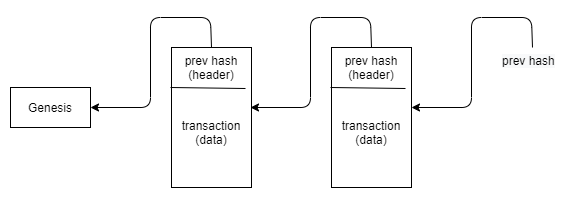
\includegraphics[width=0.5\textwidth]{CS291D-lec2-graph1.png}
		\caption{Structure of a blockchain (refer to Figure 1.11 on page 45 of~\cite{2})}
	\end{figure}
	
	\subsection{Block Structure of Bitcoin}
	
	The header of a Bitcoin block contains several fields e.g. version, a hashpointer to the previous block header, timestamp of block creation, bits, nonce, and the root of a Merkle tree
	consisting of the transactions in the data block. The data block organizes all the transactions in a Merkle tree with each leaf of the tree containing a single transaction.
	The first transaction of a block is known as a \emph{coinbase transaction}, which essentially creates new coins. The advantage of having the Merkle tree root in the header is, one can just keep 
	a hash pointer to the previous block header. It is not required to hash the entire block, and thus saves computation. The structure of Bitcoin block is demonstrated in Figure~\ref{fig:bitcoin}.
	
	
	
	
	\begin{figure}[h]
		\label{fig:bitcoin}
		\centering
		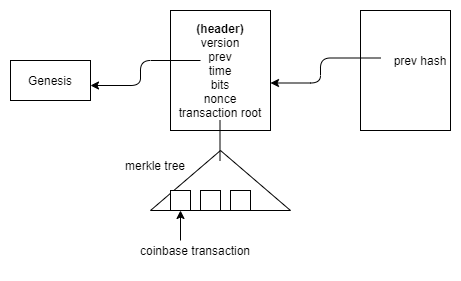
\includegraphics[width=0.5\textwidth]{CS291D-lec2-graph2.png}
		\caption{Block structure of Bitcoin}
	\end{figure}
	
	Below we introduce and discuss some key concepts related to Bitcoin.
	\begin{itemize}
		\item \textbf{UTXO:} Unspent Transaction Output.
		The UTXO model states that, a coin cannot be transferred, subdivided or combined. Whenever a coin needs to be sent to someone,
		the old coin is destroyed and a new coin is generated.
		For example, suppose Alice has 11 Bitcoins and she wants to send 9 Bitcoins to Bob. To perform this transaction, Alice first needs to destroy her 11 coins, send 9 coins to Bob, and send 2 coins to herself.
		\item \textbf{Structure of Transaction:} A transaction consists of an id, the type of the transaction, the set of input coins, and the set of output coins. The input coins are represented by the transaction id and index in which it was generated. The output coins contain the recipient's address and number of coins to be sent to each recipient. Finally, a transaction must contain the signature of the owner of the consumed coins. The structure of a transaction is depicted in Figure~\ref{fig:transaction}.
		A transaction is valid if the following three conditions hold:
		\begin{enumerate}
			\item Consumed coins are valid, i.e. it is owned by the signer and has not been spent yet.
			\item Total value out = Total value in
			\item Signed by the owner of consumed coins
		\end{enumerate}
		
		\begin{figure}[h]
			\label{fig:transaction}
			\centering
			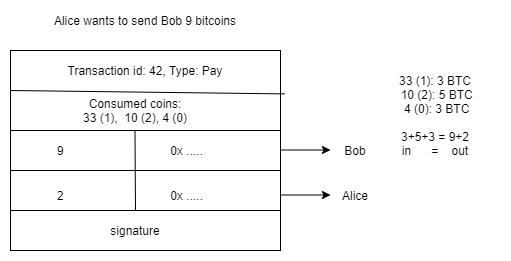
\includegraphics[width=0.5\textwidth]{CS291D-lec2-graph3.png}
			\caption{Structure of a transaction
				(refer to Figure 1.13 on page 47 of \cite{2})}
		\end{figure}           
		
		
		
		\item \textbf{Bitcoin Script}
		A bitcoin script is a non-Turing complete script programming language that runs on a stack machine. It is designed to run in a very short period of time. Bitcoin script supports many programming language constructs and cryptographic primitives. A comprehensive list of the operations supported by Bitcoin script is available in \cite{1}.
		
		
		\item \textbf{Pay to Public Key Hash(P2PKH):} This policy actually defines how addresses are generated in Bitcoin. In order to send any coin, it must be sent to the recipient's address. In Bitcoin, the SHA256 hash of the recipient's public key acts as the address. 
		Let us again consider the example where Alice has 11 Bitcoins and she wants to send 9 Bitcoins to Bob. The transaction takes place in the following steps: 
		\begin{enumerate}
			\item Bob generates his public key, secret key pair: $(\text{PK}_{B},\text{SK}_{B})$ := Generate($1^\lambda$)
			\item Bob generates his address by taking hash of his public key: $\text{Addr}_{B}$ := Hash($\text{PK}_{B}$)
			\item Bob sends  $\text{Addr}_{B}$ to Alice
			\item Alice creates the transaction
		\end{enumerate}
		After the transaction is complete, Bob can spend his UTXO referring to the transaction.
	\end{itemize}
	
	The following two design choices make the distributed ledger tamper-proof and more secure: 
	\begin{enumerate}
		\item Alice specifies the address of Bob (Hash($\text{PK}_{B}$)) in the transaction rather than Bob's actual public key.
		\item No adversary can change the recipient address ($\text{Addr}_{B}$) to steal the fund, because the transaction is signed by Alice. Any such tampering will be detectable using bitcoin script.
	\end{enumerate}
	
	\section*{References}
	\beginrefs
	\bibentry{1}
	``Script - Bitcoin wiki'' url:
	{\it https://en.bitcoin.it/wiki/Script}
	
	\bibentry{2}
	Narayanan, Arvind and Bonneau, Joseph and Felten, Edward and Miller, Andrew and Goldfeder, Steven,
	``Bitcoin and cryptocurrency technologies: a comprehensive introduction", 2016, Princeton University Press
	
	
	
	\endrefs
\end{document}
